\documentclass[10pt,a4paper]{article}
\usepackage[
  driver=xetex,
  paper=a4paper,
  layout=a4paper,
  margin=0mm,
  marginparwidth=0mm,
  marginparsep=0mm,
  % top=-15mm,
  % left=-15mm,
  % right=-15mm,
  % bottom=-15mm,
  nohead]{geometry}
\usepackage{tikz}
\usetikzlibrary{calc}
\usepackage{graphicx}
\begin{document}


%%content%%
\begin{tikzpicture}[overlay,remember picture]\node[anchor=north west,xshift=-005mm,yshift=+005.00mm] at (current page.north west){\includegraphics[width=76.75mm,height=110mm,angle=-90,page=4]{../16-page-booklet.pdf}};\end{tikzpicture}
\begin{tikzpicture}[overlay,remember picture]\node[anchor=north west,xshift=-005mm,yshift=-071.75mm] at (current page.north west){\includegraphics[width=76.75mm,height=110mm,angle=-90,page=13]{../16-page-booklet.pdf}};\end{tikzpicture}
\begin{tikzpicture}[overlay,remember picture]\node[anchor=north west,xshift=-005mm,yshift=-148.50mm] at (current page.north west){\includegraphics[width=76.75mm,height=110mm,angle=-90,page=16]{../16-page-booklet.pdf}};\end{tikzpicture}
\begin{tikzpicture}[overlay,remember picture]\node[anchor=north west,xshift=-005mm,yshift=-225.25mm] at (current page.north west){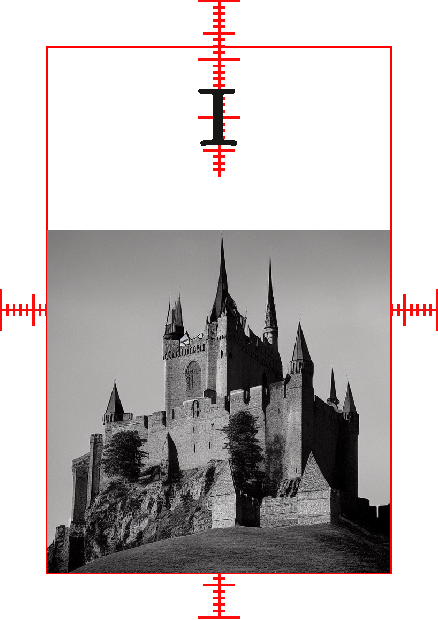
\includegraphics[width=76.75mm,height=110mm,angle=-90,page=1]{../16-page-booklet.pdf}};\end{tikzpicture}

\end{document}
